% GNUPLOT: LaTeX picture with Postscript
\documentclass{minimal}
% Set font size
\makeatletter
\def\@ptsize{0}
\InputIfFileExists{size10.clo}{}{%
   \GenericError{(gnuplot) \space\space\space\@spaces}{%
      Gnuplot Error: File `size10.clo' not found! Could not set font size%
   }{See the gnuplot documentation for explanation.%
   }{For using a font size a file `size<fontsize>.clo' has to exist.
        Falling back ^^Jto default fontsize 10pt.}%
  \def\@ptsize{0}
  \input{size10.clo}%
}%
\makeatother
% Load packages
\usepackage{graphicx}
\usepackage{color}
\makeatletter
% Select an appropriate default driver (from TeXLive graphics.cfg)
\begingroup
  \chardef\x=0 %
  % check pdfTeX
  \@ifundefined{pdfoutput}{}{%
    \ifcase\pdfoutput
    \else
      \chardef\x=1 %
    \fi
  }%
  % check VTeX
  \@ifundefined{OpMode}{}{%
    \chardef\x=2 %
  }%
\expandafter\endgroup
\ifcase\x
  % default case
  \PassOptionsToPackage{dvips}{geometry}
\or
  % pdfTeX is running in pdf mode
  \PassOptionsToPackage{pdftex}{geometry}
\else
  % VTeX is running
  \PassOptionsToPackage{vtex}{geometry}
\fi
\makeatother
% Set papersize
\usepackage[papersize={1080.00bp,252.00bp},text={1080.00bp,252.00bp}]{geometry}
% No page numbers and no paragraph indentation
\pagestyle{empty}
\setlength{\parindent}{0bp}%
% Load configuration file
\InputIfFileExists{gnuplot.cfg}{%
  \typeout{Using configuration file gnuplot.cfg}%
}{%
 \typeout{No configuration file gnuplot.cfg found.}%
}%
%
\begin{document}
\begingroup
  \makeatletter
  \providecommand\color[2][]{%
    \GenericError{(gnuplot) \space\space\space\@spaces}{%
      Package color not loaded in conjunction with
      terminal option `colourtext'%
    }{See the gnuplot documentation for explanation.%
    }{Either use 'blacktext' in gnuplot or load the package
      color.sty in LaTeX.}%
    \renewcommand\color[2][]{}%
  }%
  \providecommand\includegraphics[2][]{%
    \GenericError{(gnuplot) \space\space\space\@spaces}{%
      Package graphicx or graphics not loaded%
    }{See the gnuplot documentation for explanation.%
    }{The gnuplot epslatex terminal needs graphicx.sty or graphics.sty.}%
    \renewcommand\includegraphics[2][]{}%
  }%
  \providecommand\rotatebox[2]{#2}%
  \@ifundefined{ifGPcolor}{%
    \newif\ifGPcolor
    \GPcolortrue
  }{}%
  \@ifundefined{ifGPblacktext}{%
    \newif\ifGPblacktext
    \GPblacktextfalse
  }{}%
  % define a \g@addto@macro without @ in the name:
  \let\gplgaddtomacro\g@addto@macro
  % define empty templates for all commands taking text:
  \gdef\gplbacktext{}%
  \gdef\gplfronttext{}%
  \makeatother
  \ifGPblacktext
    % no textcolor at all
    \def\colorrgb#1{}%
    \def\colorgray#1{}%
  \else
    % gray or color?
    \ifGPcolor
      \def\colorrgb#1{\color[rgb]{#1}}%
      \def\colorgray#1{\color[gray]{#1}}%
      \expandafter\def\csname LTw\endcsname{\color{white}}%
      \expandafter\def\csname LTb\endcsname{\color{black}}%
      \expandafter\def\csname LTa\endcsname{\color{black}}%
      \expandafter\def\csname LT0\endcsname{\color[rgb]{1,0,0}}%
      \expandafter\def\csname LT1\endcsname{\color[rgb]{0,1,0}}%
      \expandafter\def\csname LT2\endcsname{\color[rgb]{0,0,1}}%
      \expandafter\def\csname LT3\endcsname{\color[rgb]{1,0,1}}%
      \expandafter\def\csname LT4\endcsname{\color[rgb]{0,1,1}}%
      \expandafter\def\csname LT5\endcsname{\color[rgb]{1,1,0}}%
      \expandafter\def\csname LT6\endcsname{\color[rgb]{0,0,0}}%
      \expandafter\def\csname LT7\endcsname{\color[rgb]{1,0.3,0}}%
      \expandafter\def\csname LT8\endcsname{\color[rgb]{0.5,0.5,0.5}}%
    \else
      % gray
      \def\colorrgb#1{\color{black}}%
      \def\colorgray#1{\color[gray]{#1}}%
      \expandafter\def\csname LTw\endcsname{\color{white}}%
      \expandafter\def\csname LTb\endcsname{\color{black}}%
      \expandafter\def\csname LTa\endcsname{\color{black}}%
      \expandafter\def\csname LT0\endcsname{\color{black}}%
      \expandafter\def\csname LT1\endcsname{\color{black}}%
      \expandafter\def\csname LT2\endcsname{\color{black}}%
      \expandafter\def\csname LT3\endcsname{\color{black}}%
      \expandafter\def\csname LT4\endcsname{\color{black}}%
      \expandafter\def\csname LT5\endcsname{\color{black}}%
      \expandafter\def\csname LT6\endcsname{\color{black}}%
      \expandafter\def\csname LT7\endcsname{\color{black}}%
      \expandafter\def\csname LT8\endcsname{\color{black}}%
    \fi
  \fi
  \setlength{\unitlength}{0.0500bp}%
  \begin{picture}(21600.00,5040.00)%
    \gplgaddtomacro\gplbacktext{%
      \csname LTb\endcsname%
      \put(740,1234){\makebox(0,0)[r]{\strut{}-10}}%
      \put(740,1977){\makebox(0,0)[r]{\strut{}-5}}%
      \put(740,2720){\makebox(0,0)[r]{\strut{} 0}}%
      \put(740,3462){\makebox(0,0)[r]{\strut{} 5}}%
      \put(740,4205){\makebox(0,0)[r]{\strut{} 10}}%
      \put(860,440){\makebox(0,0){\strut{}-2.0e+05}}%
      \put(2112,440){\makebox(0,0){\strut{}-1.0e+05}}%
      \put(3365,440){\makebox(0,0){\strut{}0.0e+00}}%
      \put(4617,440){\makebox(0,0){\strut{}1.0e+05}}%
      \put(5869,440){\makebox(0,0){\strut{}2.0e+05}}%
      \put(160,2719){\rotatebox{-270}{\makebox(0,0){\strut{}$S_d$}}}%
      \put(3364,140){\makebox(0,0){\strut{}$\gamma$}}%
    }%
    \gplgaddtomacro\gplfronttext{%
      \colorrgb{1.00,1.00,1.00}%
      \put(4966,4636){\makebox(0,0)[r]{\strut{}mean $\gamma$}}%
      \csname LTb\endcsname%
      \put(6364,640){\makebox(0,0)[l]{\strut{} 0}}%
      \put(6364,1333){\makebox(0,0)[l]{\strut{} 1e-07}}%
      \put(6364,2026){\makebox(0,0)[l]{\strut{} 2e-07}}%
      \put(6364,2719){\makebox(0,0)[l]{\strut{} 3e-07}}%
      \put(6364,3412){\makebox(0,0)[l]{\strut{} 4e-07}}%
      \put(6364,4105){\makebox(0,0)[l]{\strut{} 5e-07}}%
      \put(6364,4799){\makebox(0,0)[l]{\strut{} 6e-07}}%
    }%
    \gplgaddtomacro\gplbacktext{%
      \csname LTb\endcsname%
      \put(7940,1234){\makebox(0,0)[r]{\strut{}-10}}%
      \put(7940,1977){\makebox(0,0)[r]{\strut{}-5}}%
      \put(7940,2720){\makebox(0,0)[r]{\strut{} 0}}%
      \put(7940,3462){\makebox(0,0)[r]{\strut{} 5}}%
      \put(7940,4205){\makebox(0,0)[r]{\strut{} 10}}%
      \put(8060,440){\makebox(0,0){\strut{}-2.0e+05}}%
      \put(9312,440){\makebox(0,0){\strut{}-1.0e+05}}%
      \put(10565,440){\makebox(0,0){\strut{}0.0e+00}}%
      \put(11817,440){\makebox(0,0){\strut{}1.0e+05}}%
      \put(13069,440){\makebox(0,0){\strut{}2.0e+05}}%
      \put(7360,2719){\rotatebox{-270}{\makebox(0,0){\strut{}$S_d$}}}%
      \put(10564,140){\makebox(0,0){\strut{}$\beta$}}%
    }%
    \gplgaddtomacro\gplfronttext{%
      \colorrgb{1.00,1.00,1.00}%
      \put(12166,4636){\makebox(0,0)[r]{\strut{}mean $\beta$}}%
      \csname LTb\endcsname%
      \put(13564,640){\makebox(0,0)[l]{\strut{} 0}}%
      \put(13564,1333){\makebox(0,0)[l]{\strut{} 2e-07}}%
      \put(13564,2026){\makebox(0,0)[l]{\strut{} 4e-07}}%
      \put(13564,2719){\makebox(0,0)[l]{\strut{} 6e-07}}%
      \put(13564,3412){\makebox(0,0)[l]{\strut{} 8e-07}}%
      \put(13564,4105){\makebox(0,0)[l]{\strut{} 1e-06}}%
      \put(13564,4799){\makebox(0,0)[l]{\strut{} 1.2e-06}}%
    }%
    \gplgaddtomacro\gplbacktext{%
      \csname LTb\endcsname%
      \put(15140,1234){\makebox(0,0)[r]{\strut{}-10}}%
      \put(15140,1977){\makebox(0,0)[r]{\strut{}-5}}%
      \put(15140,2720){\makebox(0,0)[r]{\strut{} 0}}%
      \put(15140,3462){\makebox(0,0)[r]{\strut{} 5}}%
      \put(15140,4205){\makebox(0,0)[r]{\strut{} 10}}%
      \put(15260,440){\makebox(0,0){\strut{}-2.0e+05}}%
      \put(16512,440){\makebox(0,0){\strut{}-1.0e+05}}%
      \put(17765,440){\makebox(0,0){\strut{}0.0e+00}}%
      \put(19017,440){\makebox(0,0){\strut{}1.0e+05}}%
      \put(20269,440){\makebox(0,0){\strut{}2.0e+05}}%
      \put(14560,2719){\rotatebox{-270}{\makebox(0,0){\strut{}$S_d$}}}%
      \put(17764,140){\makebox(0,0){\strut{}$\alpha$}}%
    }%
    \gplgaddtomacro\gplfronttext{%
      \colorrgb{1.00,1.00,1.00}%
      \put(19366,4636){\makebox(0,0)[r]{\strut{}mean $\alpha$}}%
      \csname LTb\endcsname%
      \put(20764,640){\makebox(0,0)[l]{\strut{} 0}}%
      \put(20764,1234){\makebox(0,0)[l]{\strut{} 1e-07}}%
      \put(20764,1828){\makebox(0,0)[l]{\strut{} 2e-07}}%
      \put(20764,2422){\makebox(0,0)[l]{\strut{} 3e-07}}%
      \put(20764,3016){\makebox(0,0)[l]{\strut{} 4e-07}}%
      \put(20764,3610){\makebox(0,0)[l]{\strut{} 5e-07}}%
      \put(20764,4204){\makebox(0,0)[l]{\strut{} 6e-07}}%
      \put(20764,4799){\makebox(0,0)[l]{\strut{} 7e-07}}%
    }%
    \gplbacktext
    \put(0,0){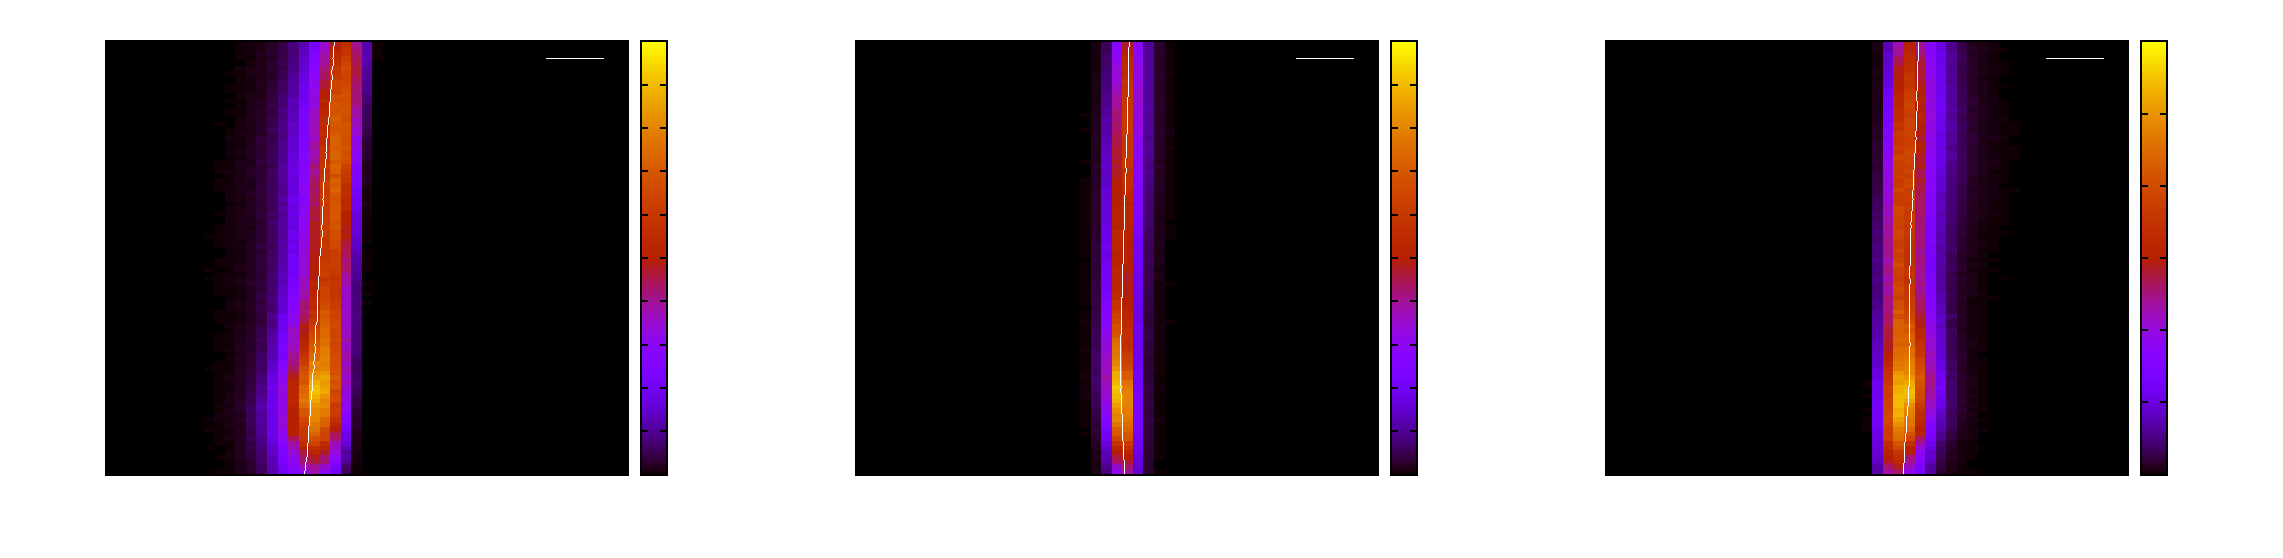
\includegraphics{R3K1_top_lambda_jpdf-inc}}%
    \gplfronttext
  \end{picture}%
\endgroup
\end{document}
